
\section*{PHỤ LỤC}
\phantomsection\addcontentsline{toc}{section}{\numberline{} PHỤ LỤC}

\subsection*{Cơ sở lý thuyết về ECG}

Tín hiệu điện tâm đồ (ECG) là một loại tín hiệu điện sinh học quan trọng, đóng vai trò quan trọng trong việc chẩn đoán các bệnh tim. Trong lĩnh vực sinh lý học, tín hiệu điện sinh học phát sinh khi các tế bào bị kích thích gây ra sự thay đổi trong điện thế màng. Hiện tượng này lan tỏa qua các vị trí lân cận, tạo ra một sự thay đổi điện thế theo thời gian. Tín hiệu này xuất phát từ các tế bào thần kinh và cơ, bao gồm cả cơ tim. Điện thế màng được tạo ra bởi sự chênh lệch nồng độ ion qua màng thấm chọn lọc của tế bào, cùng với cơ chế vận chuyển ion qua màng. Điện tâm đồ ghi lại thời gian biến đổi của tín hiệu điện thế này, không xâm lấn vào cơ thể, và được sử dụng để kiểm tra hoạt động của tim.


ECG đo sự khác biệt điện thế giữa các điện cực được đặt ở các vị trí khác nhau trên cơ thể. Điều này phản ánh hoạt động điện của tim trong một chu kỳ tim. Kĩ thuật này thường được sử dụng cùng với các xét nghiệm khác để hỗ trợ trong việc chẩn đoán và giám sát các vấn đề liên quan đến tim. ECG có khả năng phát hiện các rối loạn nhịp tim, bệnh mạch vành (sự cản trở hoặc gián đoạn trong lưu thông máu tới tim), cơn đau tim (do dòng máu bị chặn đột ngột), cũng như các vấn đề về cơ tim. Nó cũng có thể được sử dụng để theo dõi người có triệu chứng và vấn đề về tim như đau ngực, nhịp tim không đều, chóng mặt và khó thở.


Một loạt dữ liệu ECG có thể được thu thập theo thời gian để giám sát tình trạng tim của người đã được chẩn đoán mắc bệnh tim hoặc đang sử dụng các loại thuốc có thể ảnh hưởng đến tim. Điều này giúp cho việc quản lý và điều trị các bệnh tim trở nên hiệu quả hơn.


\subsection*{Công cụ sử dụng}


\subsubsection*{PlantUML}

\begin{enumerate}[a)]



  \item  Giới thiệu công cụ


\begin{figure}[H]
  \centering
  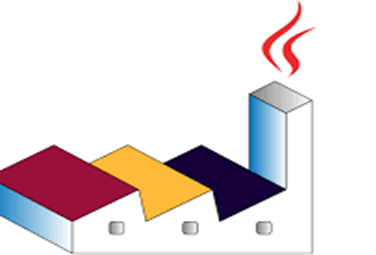
\includegraphics[width=10cm,height=8cm]{Images/appendix/plantuml.png}
  \caption[PlantUML]{\bfseries \fontsize{12pt}{0pt}
  \selectfont PlantUML}
  \label{plantuml} %đặt tên cho ảnh
\end{figure}


PlantUML là công cụ open-source, miễn phí cho phép convert những dòng code sang dạng biểu đồ UML, nó sẽ thể hiện 1 cách rõ ràng khi nhìn vào dòng code và dễ dàng triển khai


Ưu Điểm
\begin{adjustwidth}{2em}{}
  \begin{itemize}
      \item Kích thước nhẹ nên dễ dàng gửi cho người gửi.
  
      \item 	Miễn phí
      \item 	Nếu tích hợp vào dự án sử dụng git thì vì có thể review chéo, cùng xây dựng UML trong team được.
      \item 	Export ra ảnh.
      \item 	Tự động điều chỉnh vị trí các thành phần, không cần căn chỉnh
      \item 	PlantUML vẽ được hầu hết các sơ đồ UML: Sequence Diagram, Use Case Diagram, Class Diagram, Activity Diagram, Component Diagram, ...
      
  \end{itemize}
\end{adjustwidth}




\item Cách cài đặt



PlantUML chạy trên nền tảng java

Dùng extention của Visual Studio Code

Các file để vẽ UML sẽ có đuôi: *.wsd, *.pu, *.puml, *.plantuml, *.iuml


\item  Một số câu lệnh thông dụng


Cấu trúc:

\begin{lstlisting}

@startuml


@enduml

\end{lstlisting}



\textbf{Khai báo thành phần}


Để khai báo các thành phần, sử dụng các keyword

\begin{adjustwidth}{2em}{}
\begin{itemize}
  \item	actor
  \item	boundary
  \item	control
  \item	entity
  \item	database
  \item	collections
  
\end{itemize}
\end{adjustwidth}


\begin{figure}[H]
  \centering
  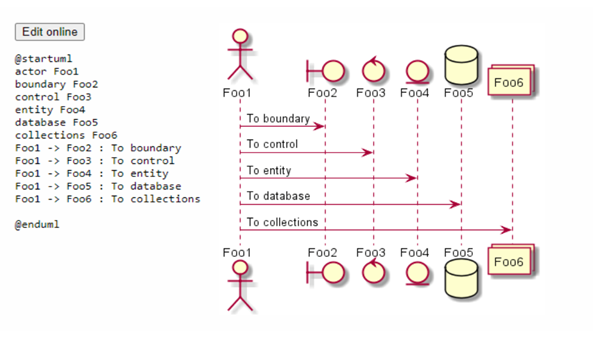
\includegraphics[width=10cm,height=8cm]{Images/appendix/plantuml_object.png}
  \caption[Hình ảnh các đối tượng]{\bfseries \fontsize{12pt}{0pt}
  \selectfont Hình ảnh các đối tượng}
  \label{plantuml_object} %đặt tên cho ảnh
\end{figure}


\textbf{Nhóm các message}

\begin{adjustwidth}{2em}{}
  \begin{itemize}
    \item alt/else
    \item opt
    \item loop
    \item par
    \item break
    \item critical
    \item group: 1 text bất kỳ, nó sẽ được hiển thị ở header của group khi đóng nhóm dùng end. Các nhóm cũng có thể lồng với nhau
    
    
  \end{itemize}
  \end{adjustwidth}


  \begin{figure}[H]
    \centering
    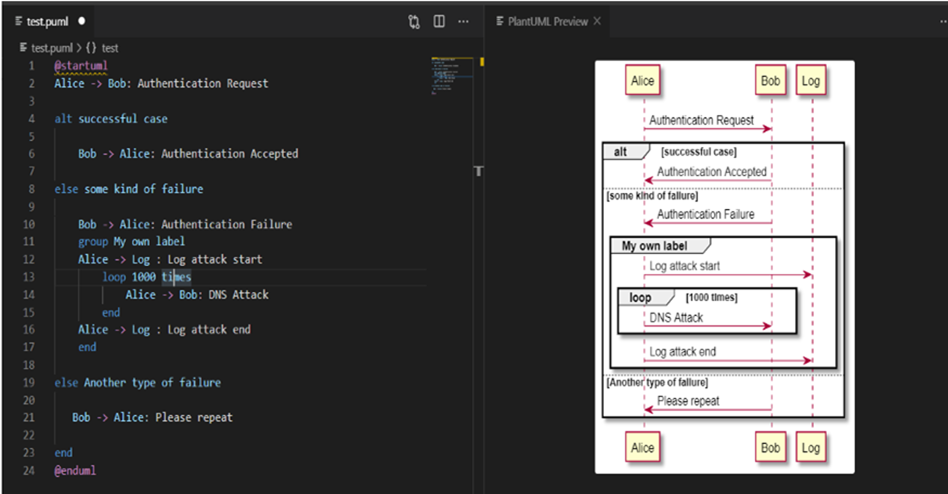
\includegraphics[scale=0.5]{Images/appendix/plantuml_loops.png}
    \caption[Các vòng lặp trong UML]{\bfseries \fontsize{12pt}{0pt}
    \selectfont Các vòng lặp trong UML}
    \label{plantuml_object} %đặt tên cho ảnh
  \end{figure}


  \textbf{Notes trên messages}
  
  \begin{figure}[H]
    \centering
    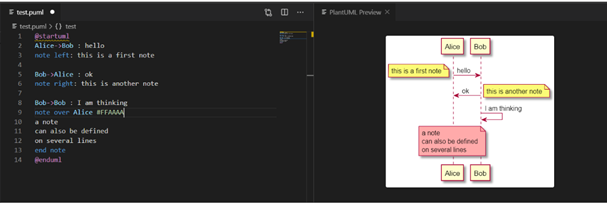
\includegraphics[width=10cm,height=8cm]{Images/appendix/plantuml_note.png}
    \caption[Các kiểu note]{\bfseries \fontsize{12pt}{0pt}
    \selectfont Các kiểu note}
    \label{plantuml_object} %đặt tên cho ảnh
  \end{figure}


  
\begin{adjustwidth}{2em}{}
  \begin{itemize}

    \item Note left để note nằm bên trái.
    \item Note right để note nằm bên phải.
    \item Note over để note over (nằm giữa).
    \item End note để kết thúc note có nhiều dòng.
    \item	Ngoài ra có thể thay đổi màu backgroup của note (mặc định màu vàng)
    
    
  \end{itemize}
  \end{adjustwidth}

  \textbf{Ví dụ minh họa:}

  \begin{figure}[H]
    \centering
    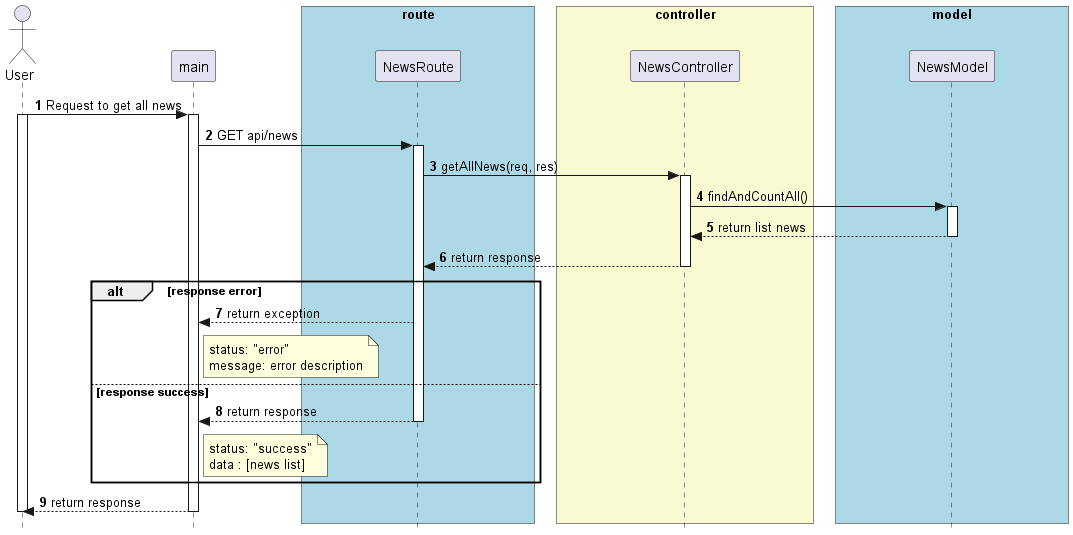
\includegraphics[width=10cm,height=8cm]{Images/server/sequence/server/getAllNews.png}
    \caption[Ví dụ minh họa]{\bfseries \fontsize{12pt}{0pt}
    \selectfont Ví dụ minh họa}
    \label{plantuml_object} %đặt tên cho ảnh
  \end{figure}



\begin{lstlisting}

@startuml

skinparam style strictuml
skinparam lifelineStrategy solid
skinparam ParticipantPadding 70
skinparam BoxPadding 10

autonumber

actor User as User
participant main as main

box "route" #lightBlue
participant NewsRoute as NewsRoute
end box

box "controller" #LightGoldenRodYellow
participant NewsController as NewsController
end box

box "model" #lightBlue
participant NewsModel as NewsModel
end box

User -> main: Request to get all news
activate User
activate main
main -> NewsRoute: GET api/news
activate NewsRoute

NewsRoute -> NewsController: getAllNews(req, res)
activate NewsController

NewsController -> NewsModel: findAndCountAll()
activate NewsModel
NewsModel --> NewsController: return list news
deactivate NewsModel
NewsController --> NewsRoute: return response
deactivate NewsController

alt response error
  NewsRoute --> main: return exception
  note right of main
    status: "error"
    message: error description
  end note
else response success
  NewsRoute --> main: return response
    deactivate NewsRoute

  note right of main
    status: "success"
    data : [news list]
  end note
end
main --> User: return response
deactivate main
deactivate User

@enduml

\end{lstlisting}

\end{enumerate}


\subsubsection*{Github}

\begin{enumerate}[a)]
  \item Giới thiệu chung
  
  GitHub là một hệ thống dịch vụ lưu trữ mã nguồn trực tuyến được sử dụng rộng rãi bởi các lập trình viên trên toàn thế giới. GitHub cung cấp một nơi để lưu trữ mã nguồn và quản lý các dự án phần mềm. Nó cho phép người dùng tạo các kho lưu trữ để chia sẻ, quản lý, và phát triển mã nguồn một cách dễ dàng.

  \item Các tính năng
  
Lưu trữ mã nguồn: GitHub cho phép người dùng tạo các kho lưu trữ để lưu trữ mã nguồn của dự án. Những kho lưu trữ này có thể được chia sẻ với người dùng khác để họ có thể đóng góp vào dự án.


Quản lý phiên bản: GitHub cho phép người dùng theo dõi các thay đổi trong mã nguồn và quản lý phiên bản. Người dùng có thể xem các sửa đổi được thực hiện bởi các thành viên khác và đối chiếu với phiên bản trước để kiểm tra xem sự thay đổi có đáng tin cậy hay không.


Hỗ trợ cho các dự án lớn: GitHub cung cấp các công cụ để quản lý các dự án phần mềm lớn với nhiều người đóng góp. Nó cho phép người dùng tạo các nhánh để làm việc trên các tính năng riêng lẻ và sau đó hợp nhất chúng với nhau khi chúng đã được hoàn thiện.


Hỗ trợ cho các công cụ phát triển phần mềm khác: GitHub tích hợp với các công cụ phát triển phần mềm phổ biến như Visual Studio Code, Eclipse, Sublime Text, và nhiều công cụ khác để tạo ra môi trường phát triển toàn diện cho các lập trình viên.



  \item Cách sử dụng
  
Đăng ký tài khoản: để có thể sử dụng các tính năng của GitHub, người dùng cần truy cập trang chủ theo đường link https://github.com/ để tiến hành đăng ký tài khoản sử dụng.


Tạo kho lưu trữ: Người dùng có thể tạo các kho lưu trữ để lưu trữ mã nguồn và quản lý dự án của mình.


	Đóng góp vào dự án khác: Người dùng có thể đóng góp vào dự án khác bằng cách tạo các yêu cầu kéo (pull requests) và phản hồi (feedback) cho các lập trình viên khác.


	Quản lý phiên bản: Người dùng có thể quản lý phiên bản của dự án bằng cách sử dụng các tính năng của GitHub như nhánh, tạo nhánh mới, hợp nhất nhánh.


Hỗ trợ cho các công cụ phát triển phần mềm: GitHub tích hợp với các công cụ phát triển phần mềm như Visual Studio Code, Eclipse, Sublime Text, và nhiều công cụ khác để cung cấp cho người dùng một môi trường phát triển toàn diện và thuận tiện.


Theo dõi các dự án: Người dùng có thể theo dõi các dự án mà họ quan tâm bằng cách theo dõi kho lưu trữ của dự án đó trên GitHub.


Hỗ trợ cho các dự án công cộng: GitHub cũng cung cấp tính năng cho phép người dùng tạo các dự án công cộng để chia sẻ mã nguồn với cộng đồng lập trình viên.


Học tập và chia sẻ kiến thức: Ngoài việc sử dụng GitHub để lưu trữ và quản lý mã nguồn, người dùng cũng có thể sử dụng GitHub để học tập và chia sẻ kiến thức. Các kho lưu trữ công khai có thể cung cấp các tài liệu và hướng dẫn cho các lập trình viên mới.

  
\end{enumerate}

\subsection*{Đường dẫn mã nguồn}

\clearpage